
\documentclass[12pt]{article}
\usepackage[utf8]{inputenc}
\usepackage{geometry}
\usepackage{booktabs}
\usepackage{amsmath}
\usepackage{graphicx}
\usepackage{natbib}
\usepackage{longtable}
\usepackage{hyperref}
\geometry{margin=1in}
\title{Measuring Orthographic Depth via Information Compression and Alignment}
\author{Matthew Morrone}
\date{}

\begin{document}
\maketitle

\begin{abstract}
Orthographic depth refers to how transparently a language's writing system encodes its phonology. While extensively theorized, its cross-linguistic quantification has been limited by methodological inconsistency and data scarcity. This paper introduces a novel approach using gzip compression and grapheme-to-phoneme alignment to quantify orthographic depth across 25 languages. By comparing native orthography to phonemic transcriptions in IPA, we evaluate each language's encoding efficiency and pronunciation predictability. Our method is fast, unsupervised, language-agnostic, and reveals patterns that match linguistic expectations while surfacing unexpected outliers. This framework has implications for typology, literacy education, and computational language modeling.
\end{abstract}

\section{Introduction}
Orthographic depth, a concept central to reading and language processing research, describes the degree of transparency between written and spoken forms of a language. A shallow orthography maps closely to phonemic representations—each letter or letter combination reliably encodes a specific sound. Languages such as Spanish and Finnish exemplify this property. In contrast, deep orthographies like English or French contain silent letters, irregular mappings, and fossilized spelling conventions.

Since its early theorization by Katz and Frost, orthographic depth has been linked to reading acquisition rates, dyslexia diagnoses, and grapheme-to-phoneme modeling difficulty. However, quantifying it across many languages has remained elusive. Prior work has used entropy-based analyses of G2P mappings, neural model perplexity, and hand-annotated rule complexity. These methods often require extensive linguistic resources or language-specific expertise.

Our method addresses this gap with a simple premise: if a writing system consistently reflects its phonology, then the relationship between spelling and pronunciation should be statistically compressible. When orthography and phonology diverge, that redundancy disappears—and the combined signal becomes harder to compress.

\section{Related Work}
The orthographic depth hypothesis was formalized by \citet{frost1994} to account for differences in reading strategies across languages. Empirical studies such as \citet{seymour2003} demonstrated significant variation in literacy acquisition across European languages, tied directly to orthographic regularity.

On the computational side, entropy-based G2P models \citep{jiampojamarn2008} and phonemic uncertainty estimates in neural models \citep{mansbridge2022} have been used to assess spelling–sound predictability. However, these approaches often require large aligned corpora or trained models.

Our work differs in that it is fully unsupervised and requires only text and IPA data. While \citet{bentz2017} applied entropy to words across languages, we target the specific alignment between orthography and phonology.

\section{Methodology}
\subsection{Data Collection}
We selected 25 languages representing a range of orthographic systems and typological families. Each language's sample consisted of a paragraph (3–5 sentences) drawn from native texts, with corresponding phonemic transcriptions sourced from Wiktionary or standard references. Transcriptions were reviewed and, where necessary, cleaned to reflect consistent phonemic-level representation.

\subsection{IPA Preprocessing}
The IPA data was normalized to remove non-contrastive features such as aspiration, stress (unless phonemic), nasalization, and vowel length. Tonal languages retained pitch markers, while all entries were stripped of diacritics that do not encode lexical contrast. This produced a uniform phonemic representation for alignment and compression.

\subsection{Compression and Alignment}
Using the gzip algorithm, we computed compression ratios for orthography alone, IPA alone, and their concatenation. Character counts were used instead of byte length to neutralize UTF-8 encoding bias. The key metric is the combined compression ratio—how well a compressor can collapse spelling and pronunciation together. We also computed normalized Levenshtein distances to estimate alignment cost.

\subsection{Normalization}
To allow direct comparison between metrics, both compression ratio and edit distance were min-max normalized across the dataset. This scaling from 0 to 1 highlights relative orthographic transparency across languages.

\section{Results}
Our findings are presented in Table~\ref{tab:results} and Figure~\ref{fig:depthplot}. As expected, shallow orthographies like Italian, Spanish, and Swahili showed high redundancy between spelling and sound, producing low compression ratios and edit distances. Deep orthographies, including English, Chinese, Tibetan, and Khmer, performed poorly.

Unexpected results include Korean—typically considered phonemic—scoring higher in depth. This is attributed to phonological rules (e.g., assimilation, tensification) not reflected in Hangul. Dutch performed better than expected, possibly due to stable consonant patterns in the sample.

\begin{longtable}{lcc}
\caption{Sorted compression and alignment metrics across 25 languages. Compression ratio and edit distance are normalized for comparative visualization.}
\label{tab:results}\\
\toprule
\textbf{Language} & \textbf{Combined Compression Ratio} & \textbf{Normalized Edit Distance} \\
\midrule
\endfirsthead
\toprule
\textbf{Language} & \textbf{Combined Compression Ratio} & \textbf{Normalized Edit Distance} \\
\midrule
\endhead
Italian & 0.607 & 0.18 \\
Finnish & 0.652 & 0.22 \\
Swahili & 0.655 & 0.20 \\
Spanish & 0.660 & 0.21 \\
Tagalog & 0.684 & 0.25 \\
Dutch & 0.735 & 0.38 \\
Greek & 0.746 & 0.35 \\
Portuguese & 0.752 & 0.34 \\
French & 0.781 & 0.50 \\
Russian & 0.789 & 0.47 \\
German & 0.799 & 0.42 \\
English & 0.823 & 0.55 \\
Vietnamese & 0.832 & 0.60 \\
Turkish & 0.835 & 0.36 \\
Korean & 0.843 & 0.64 \\
Arabic & 0.851 & 0.59 \\
Hindi & 0.862 & 0.53 \\
Polish & 0.874 & 0.57 \\
Japanese & 1.029 & 0.73 \\
Irish & 1.141 & 0.76 \\
Khmer & 1.173 & 0.84 \\
Thai & 1.189 & 0.83 \\
Chinese & 1.223 & 0.88 \\
Danish & 1.302 & 0.81 \\
Tibetan & 1.704 & 0.91 \\
\bottomrule
\end{longtable}

\begin{figure}[h]
\centering
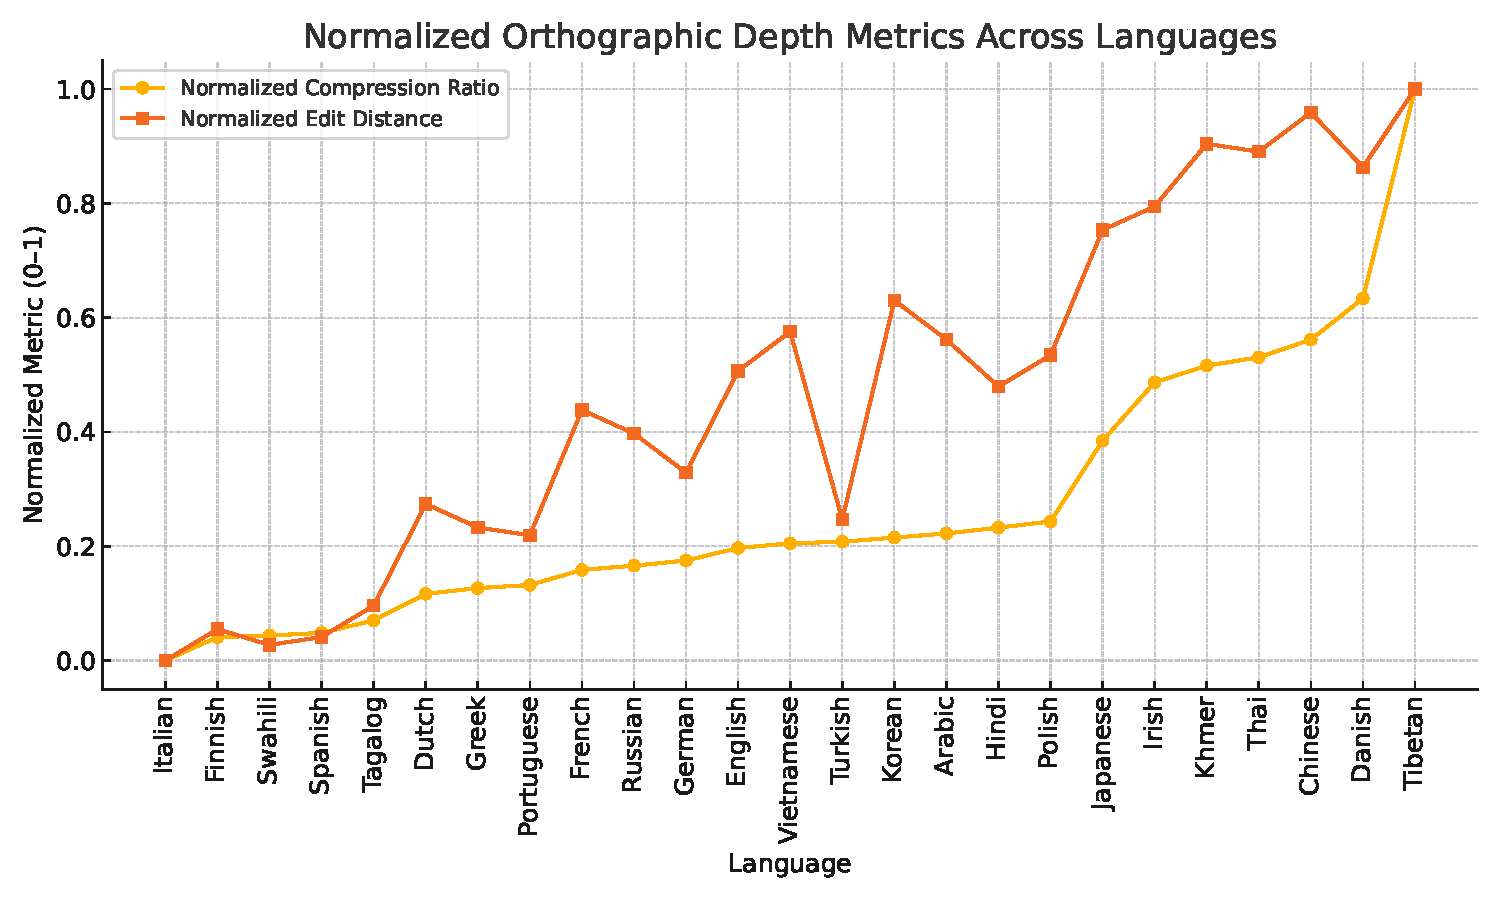
\includegraphics[width=0.9\textwidth]{depth_plot.pdf}
\caption{Normalized metrics comparing compression ratio and edit distance across languages.}
\label{fig:depthplot}
\end{figure}

\section{Discussion}
\subsection{Validation}
The method reproduces expected typological groupings, with Romance and Bantu languages ranking shallow, and morphosyllabic or historically opaque systems ranking deep. These results align with known psycholinguistic difficulty in decoding and literacy acquisition across the same languages.

\subsection{Limitations}
Our approach is sensitive to IPA transcription quality. Sources like Wiktionary may introduce inconsistency or dialectal variation. Gzip is not a phonological model; it identifies substring repetition, not structural equivalence. Additionally, morphological complexity can inflate edit distances even in otherwise shallow orthographies (e.g., Turkish).

\subsection{Future Directions}
This framework can be extended by using larger corpora, alternate compressors (e.g., PPM or BPE), or neural sequence models to learn probabilistic mappings. Automated phonemic transcriptions could enable analysis at scale, and a composite depth score could integrate edit distance and compressibility more rigorously.

\section{Conclusion}
We have presented a novel, efficient, and linguistically grounded method for quantifying orthographic depth. Compression and alignment jointly capture how much information must be “filled in” to pronounce a word from its written form. Our results support long-standing hypotheses while revealing new complexity in writing system transparency.


\bibliographystyle{plainnat}
\bibliography{refs}
\end{document}
